\section{Method}
\label{sec:meth}

We follow the notion of spatial signatures as a framework
to develop our classification.
% What SS are
This approach was developed by \cite{dab_mf_2021}, who define it as:

\newtheorem*{theorem}{}
\begin{theorem}
    A characterisation of space based on form and function designed to understand urban
environments
\end{theorem}

Spatial signatures thus provide a typology of space defined by both form and function
together, encoding both patterns of each aspect as well as the interplay between the two. 
% We focus on form only
The field of urban morphology tends to consider form only when studying urban
environments, leaving aside functional aspects such as population, amenities,
or green and blue spaces. 
%
This paper explores the form component of the spatial signatures.
Our characterisation focuses only on morphological aspects of urban
environments, thus better aligning itself with the urban morphology tradition.
% The result of our analysis is thus ``morphosignatures''
Because we follow the spatial signatures framework but focus on form-based
characters only, we call the results of our analysis, both the types we derive
and delineations we obtain, \textit{morphosignatures}.

% - spatial unit -- spatial unit criteria -- issues with available units -- proposal of
%   enclosed tessellation -- brief description and a reference to conceptual?
Spatial signatures, and morphosignatures by extension, are conceptually defined as an aggregation of granular elements into
contiguous areas based on the homogeneity of their characterisation. That
poses the subsequent methodological question: which spatial unit should be
used for developing of such characterisation? We argue the optimal unit should
be: \textit{indivisible}, so that if split into
smaller components, none of them would be enough to encode character of a
(morpho)signature;
\textit{internally consistent}, in a way that each observation reflects a single (morpho)signature type;
and geographically \textit{exhaustive}, with all the space in the area of
interest assigned into one and only one (morpho)signature.

The literature tends to be split into three groups when it comes to unit of
analysis.
%
The first relies on predefined administrative units (REF)
which, although they are convenient to source, can be counter-productive and
“obscure morphologic reality” \citep{taubenbock2019new}.
%
The second employs uniform grids, either linked to a spatial index (like hexagonal H3 grid
from \citealp{brodsky2018h3}) or to ancillary data commonly distributed on
grids (e.g. WorldPop grids as in \citealp{jochem2020}). Regular geometries are often internally
inconsistent as their definition does not reflect the spatial configuration on the
ground, thus commonly prone to the modifiable areal unit problem (MAUP,
\citealp{openshaw1981modifiable}).
%
The third and most common approach in urban morphology is to use structural
elements such as
buildings \citep{hamaina2012a}, street segments \citep{araldi2019} or plots
\citep{berghauserpont2019a} as a unit. These are closer to the underlying
entity of interest, but are not exhaustive of space as they are not
present in un-built areas. Plots would theoretically provide geographical exhaustiveness
but since their conceptual definition is not stable and geometric representation varies
\citep{kropf2018plots}, they are unfit for large scale analysis.

We follow \cite{dab_mf_2021} in adopting an alternative spatial unit named \textit{enclosed tessellation cell}
(ETC) which is defined as:

\begin{theorem}
    The portion of space that results from growing a morphological tesselation within an
enclosure delineated by a series of natural or built barriers identified from the
literature on urban form, function and perception.
\end{theorem}

The ETCs are generated in three steps illustrated on a Figure \ref{fig:et_diagram}.
First, a defined set of spatial features that divide space into smaller parts
(\ref{fig:et_diagram}A) is integrated into a single set of boundaries
(\ref{fig:et_diagram}B). Such boundaries are usually formed by linear features as street
network, railway or rivers. Second, these boundaries are used to subdivide space into
\textit{enclosures}, a smaller areas delimited from all sides by at least one boundary
feature (\ref{fig:et_diagram}C). Third, enclosures are combined with building footprints
taking the role of anchors in space and subdivided into ETCs using the morphological tesselation algorithm
\citep{fleischmann2020morphological} (\ref{fig:et_diagram}D).

\begin{figure}
    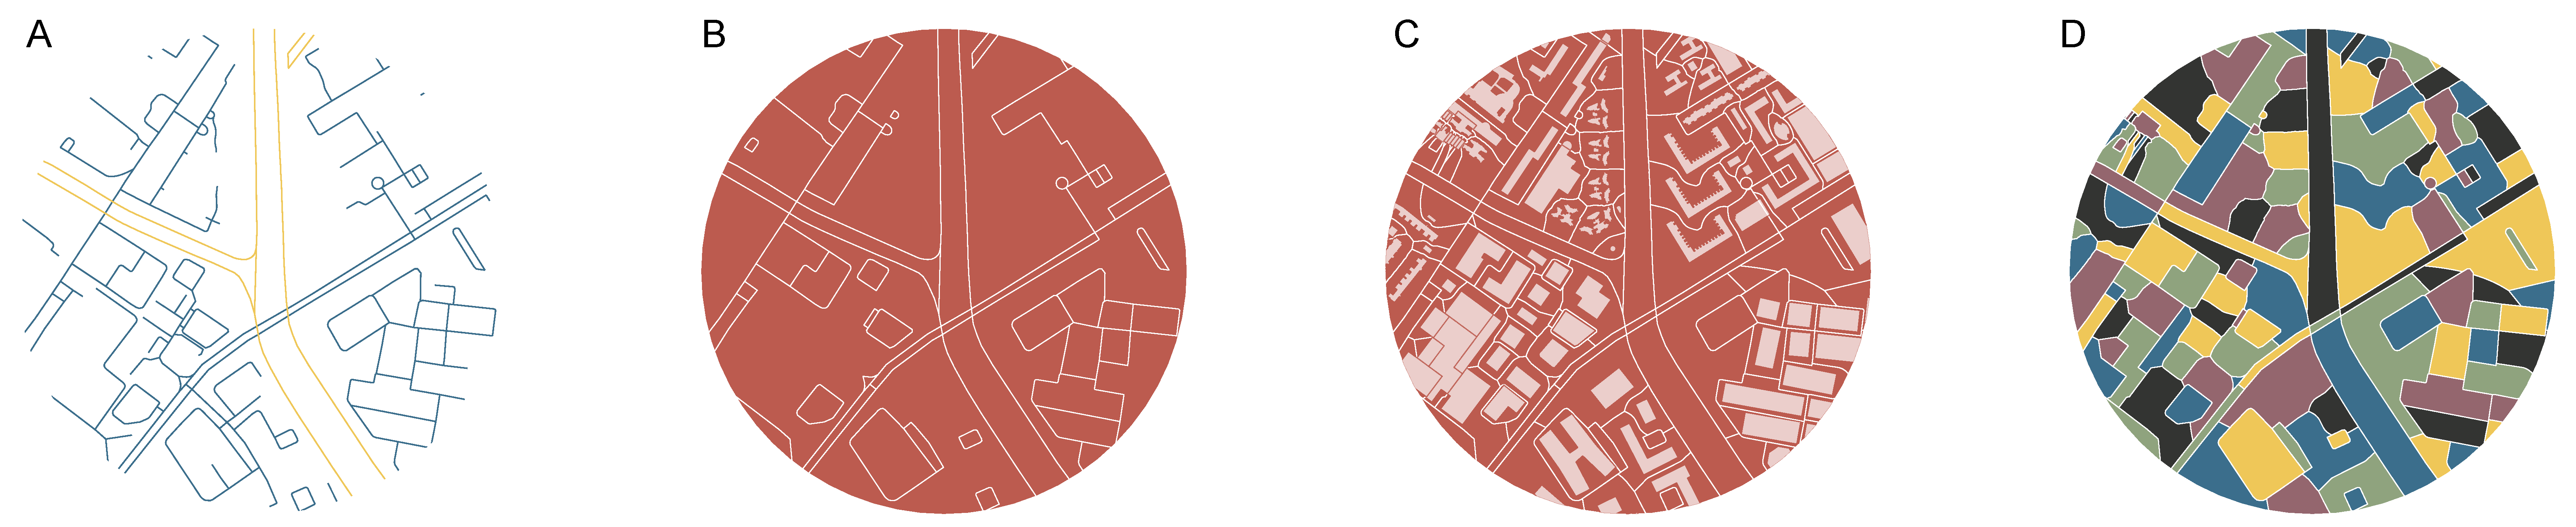
\includegraphics[width=\linewidth]{fig/et_diagram.pdf}
    \caption{Diagram illustrating the sequential steps leading to the delineation of
    enclosed tessellation. From a series of enclosing components, where blue are streets
    and yellow river banks (A), to enclosures (B), incorporation of buildings as anchors
    (C) to final tessellation cells (D).}
    \label{fig:et_diagram}
\end{figure}

Resulting ETCs are indivisible and internally consistent, as they are
linked at maximum to a single building, and exhaustive as they cover the entirety of space
thanks to contiguous geometry of enclosures. Their structure and scale adapts to the
environment and can take a form of a small-scale granular mesh in city centres of
historical origin as well as large-scale polygons encoding the vast natural open spaces.

% - morphometrics
% -- characterisation of building patterns using morphometrics
% -- the principle of inclusiveness (more better) to minimise selection bias
% - context
% -- representation of context as topological distance
% -- reflection of distribution of characters
Having ETCs, building footprints and street networks, we measure a wide range of aspects
of their spatial organisation, from dimensions and shapes of individual objects to their
spatial distribution, intensity or connectivity reflecting configuration of streets. We
call these measurements \textit{morphometric characters}. Since we do not a-priori know
which characters are determining the differences between types of urban
development the most, we aim to include a relatively large set of characters to
avoid potential selection bias, believing that further steps will be able to deal with a
larger amount of input data generated by a larger number of characters\footnote{The list
of measured morphometric characters and their implementation details are available in
the online repository at \url{https://github.com/urbangrammarai/spatial\_signatures}}. As the aim is
to use these characters to detect contiguous homogenous areas of urban form, we are more
interested in tendencies of their distributions within space. Therefore, we link all
values to ETCs and capture the distribution of each within a spatial context
around each ETC. Context here is defined as in terms of topological distance (10 steps)
between ETCs, with each one in reach being weighted by its distance to the original ETC. This
kind of aggregation is adaptive to the pattern of ETCs and reflects the higher importance
of close elements compared to more distant ones.

% - clustering & dissolution
% -- K-Means clustering of ET cells based on morphometric profile
% -- hierarchical approach - sub-dividing interesting clusters via second level K-Means
% -- aggregation of cells into form-based signatures
ETCs characterised by contextualised morphometric characters are grouped using
the K-Means algorithm, effectively deriving a typology of ETCs. Even though K-Means itself does not
contain any contiguity constraint, the design of inherently spatially autocorrelated
characters results in larger clusters that are spatially contiguous. Moreover,
this approach can be potentially applied hierarchically. When further detail
is needed, the algorithm can be run within individual
clusters. Finally, ETCs are
aggregated together based on their class, resulting in the set of spatial
morphosignature geometries, where
each contiguous area assigned the same cluster represents a single morphosignature.

% - case study - GB
We deploy this approach on the case of Great Britain, illustrating both
potential and limits of the analysis of urban form at scale.
% - data
% -- input data in general
% -- input data in the GB
% -- OS Open Map
% --- potential limitation of open data
% -- OS Open Roads
All the datasets we rely on are available openly. First, for
barriers encoding delimiters of enclosures,  we use the following: street
networks from the ``OS Open Roads'' data product,
representing street centrelines; railways from the ``OS
OpenMap - Local''; rivers from ``OS OpenRivers''; and a coastline from OS
Strategi® (REF). All these products are released by the Ordnance Survey under
an Open Government License, allowing us to release the
resulting classification as an open data product. The second input is the layer capturing
building footprints, which is again retrieved from the ``OS OpenMap - Local''. However, the
data reflect aggregated footprints and do not distinguish between individual buildings
when they are adjacent. While that is indeed a limitation, the method is designed and
tested \citep{dab_mf_2021} to be robust enough to accommodate for various
sub-optimal data sources.
